\documentclass{beamer}
\usepackage[utf8]{inputenc}

\begin{document}

\title{Electicity demand forecasting with advanced metering infrastructure}
\author{David Prentiss}
\institute{OR750-004 Fall 2018}
\date{\today}

\frame{\titlepage}

\begin{frame}
  \frametitle{Dataset}
  \begin{itemize}
    \item Advanced metering infrastructure
    \item 96 residential smart meters in the ERCOT (Texas RTO)
    \item 15-minute interval energy use
    \item Inconsistent data logging between July and November 2018
    \item No significant intervals with all meters reporting
    \item 15-minute local (zip-code) weather data
  \end{itemize}
\end{frame}

\begin{frame}
  \frametitle{Dataset}
  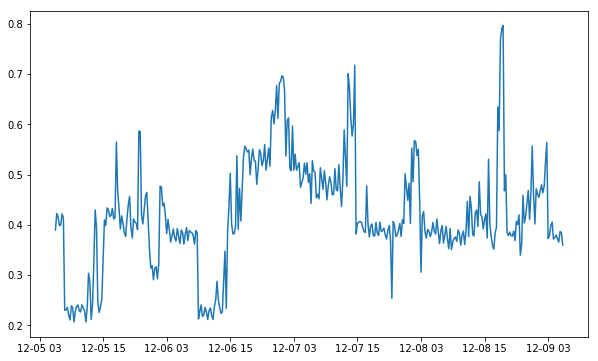
\includegraphics[width=\textwidth]{ami.png}
\end{frame}

\begin{frame}
  \frametitle{Dataset}
  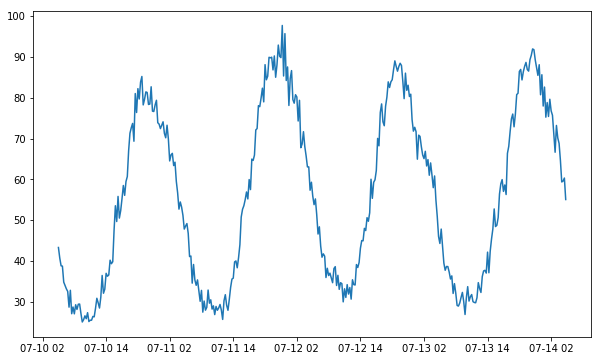
\includegraphics[width=\textwidth]{sum.png}
\end{frame}

\begin{frame}
  \frametitle{Dataset}
  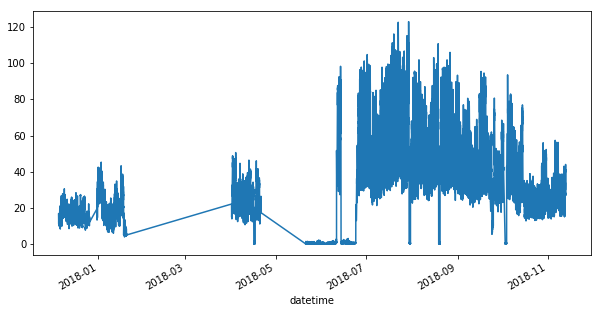
\includegraphics[width=\textwidth]{datetimesum.png}
\end{frame}

\begin{frame}
  \frametitle{Formulation}
  \begin{itemize}
    \item Forecast profile demand (sum) for 96 hours (four days)
    \item Sell appliance level load removal options (smart thermostats, etc.)
    \item Improve load-zone demand forecasting
    \item Estimate the ROI for expanding AMI profile
    \item Estimate expected value of perfect information (EVPI)
  \end{itemize}
\end{frame}

\begin{frame}
  \frametitle{Formulation}
  \begin{itemize}
    \item NaNs replaced with dataset mean
    \item \([0,1]\) scaling and mean-zero normalized
    \item Chose MSE loss function with sum reduction
    \item Focused on in-sample error while constructing model
    \item Not enough data to learn annual signals
    \item Better data will be available next year
  \end{itemize}
\end{frame}

\begin{frame}
  \frametitle{Model}
  \begin{itemize}
    \item LSTM with linear output layer
    \item 96-element input
    \item 96-element hidden state vector
    \item 384-element output layer (4 X 96 15-min intervals in 4 days)
    \item Pytorch default initialization (He)
    \item 4 LSTM layers
    \item Adam optimizer
    \item Learning rate: 0.01
    \item 500 epochs, 4 hours?
    \item Lowest MSE ~30,000
  \end{itemize}
\end{frame}

\begin{frame}
  \frametitle{Model}
  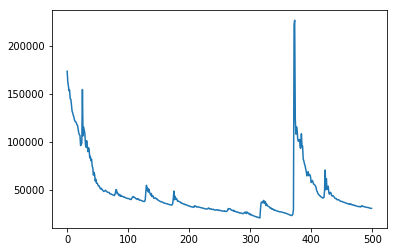
\includegraphics[width=\textwidth]{MSE.png}
\end{frame}

\begin{frame}
  \frametitle{Model}
  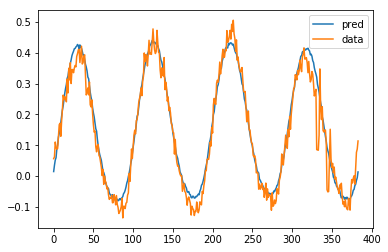
\includegraphics[width=\textwidth]{goodfit.png}
\end{frame}

\begin{frame}
  \frametitle{Model}
  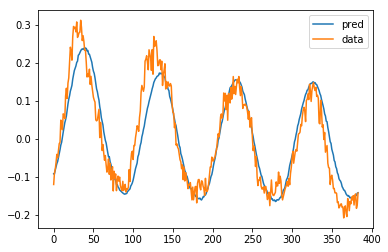
\includegraphics[width=\textwidth]{okfit.png}
\end{frame}

\begin{frame}
  \frametitle{Model}
  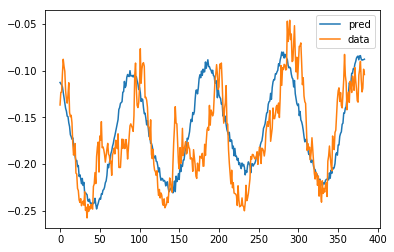
\includegraphics[width=\textwidth]{badfit.png}
\end{frame}

\begin{frame}
  \frametitle{Model}
  \begin{itemize}
    \item 4-384 elements in hidden state vector
    \item 1-24 LSTM layers
    \item SGD optimizer
    \item 0.1 - 0.001 learning rate
    \item All variants produce a noisy sinusoid with 24-hour period
  \end{itemize}
\end{frame}

\begin{frame}
  \frametitle{Model}
  \begin{itemize}
  \item Find an architecture with better in-sample performance
  \item Get access to GPUs
  \item Incorporate perfect information weather data
  \item Incorporate historical weather forecasts
  \item Attempt to predict load-zone demand
  \end{itemize}
\end{frame}

\end{document}